\documentclass{standalone}
\usepackage{tikz}
\usetikzlibrary{patterns, positioning}


\begin{document}
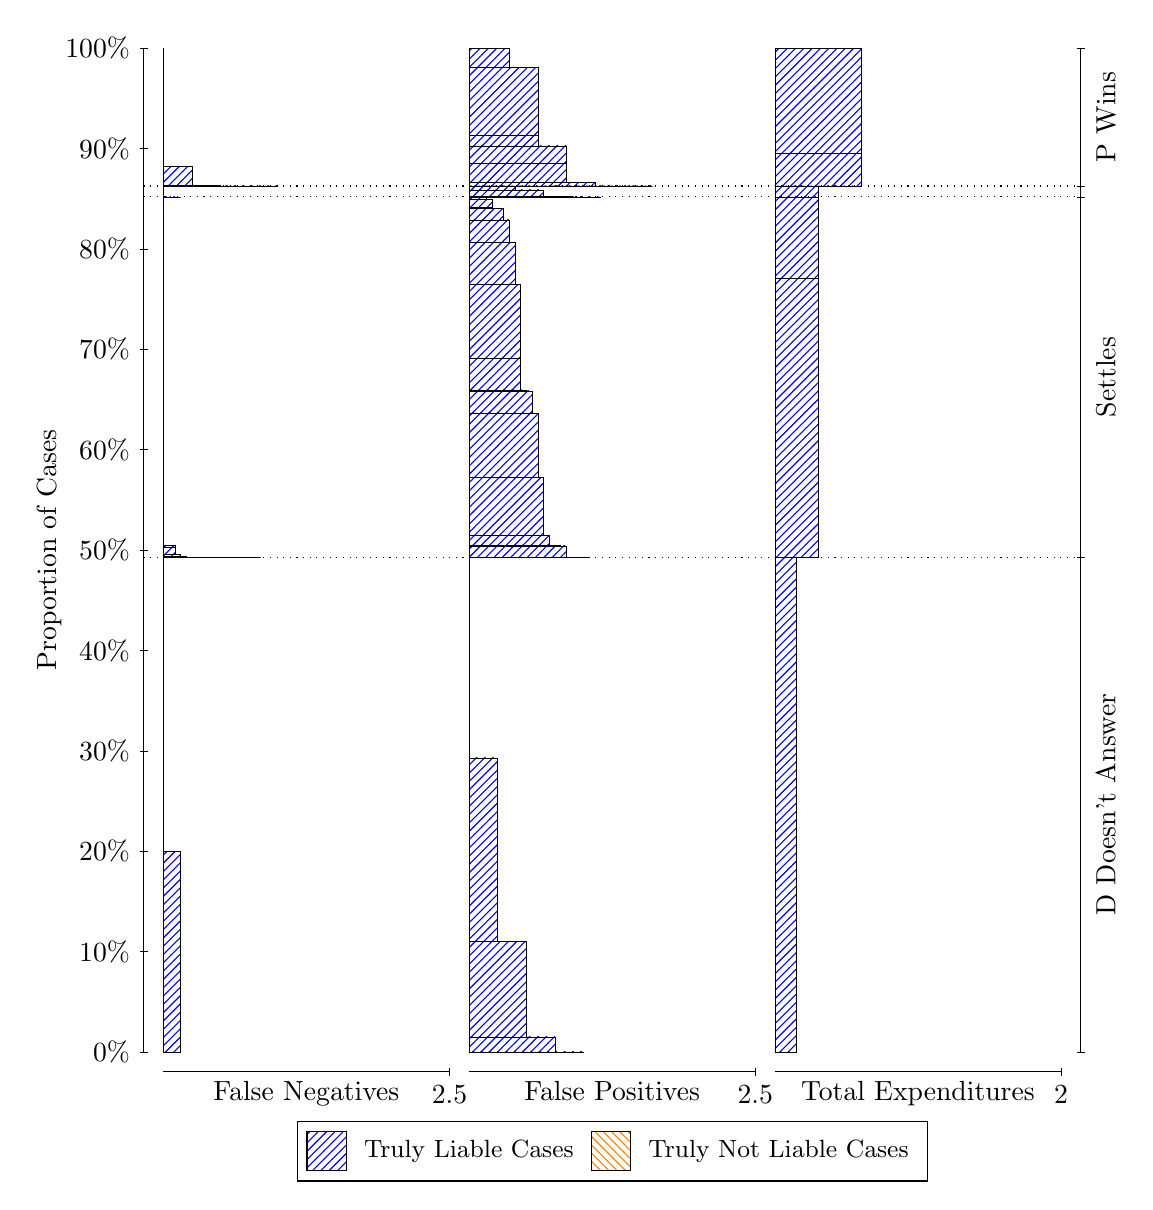
\begin{tikzpicture}
\draw[black, very thin] (1.5,1.75) -- (1.5,14.5);
\node[rotate=90, text=black, anchor=center] at (0.3, 8.125) {Proportion of Cases};
\draw[black, very thin] (1.45,1.75) -- (1.55,1.75);
\node[text=black, anchor=east] at (1.45, 1.75) {0\%};
\draw[black, very thin] (1.45,3.025) -- (1.55,3.025);
\node[text=black, anchor=east] at (1.45, 3.025) {10\%};
\draw[black, very thin] (1.45,4.3) -- (1.55,4.3);
\node[text=black, anchor=east] at (1.45, 4.3) {20\%};
\draw[black, very thin] (1.45,5.575) -- (1.55,5.575);
\node[text=black, anchor=east] at (1.45, 5.575) {30\%};
\draw[black, very thin] (1.45,6.85) -- (1.55,6.85);
\node[text=black, anchor=east] at (1.45, 6.85) {40\%};
\draw[black, very thin] (1.45,8.125) -- (1.55,8.125);
\node[text=black, anchor=east] at (1.45, 8.125) {50\%};
\draw[black, very thin] (1.45,9.4) -- (1.55,9.4);
\node[text=black, anchor=east] at (1.45, 9.4) {60\%};
\draw[black, very thin] (1.45,10.675) -- (1.55,10.675);
\node[text=black, anchor=east] at (1.45, 10.675) {70\%};
\draw[black, very thin] (1.45,11.95) -- (1.55,11.95);
\node[text=black, anchor=east] at (1.45, 11.95) {80\%};
\draw[black, very thin] (1.45,13.225) -- (1.55,13.225);
\node[text=black, anchor=east] at (1.45, 13.225) {90\%};
\draw[black, very thin] (1.45,14.5) -- (1.55,14.5);
\node[text=black, anchor=east] at (1.45, 14.5) {100\%};

\draw[black, very thin] (13.4,1.75) -- (13.4,14.5);
\draw[black, very thin] (13.35,1.75) -- (13.45,1.75);
\node[anchor=west] at (13.35, 1.75) {};
\draw[black, very thin] (13.35,8.0337) -- (13.45,8.0337);
\node[anchor=west] at (13.35, 8.0337) {};
\draw[black, very thin] (13.35,12.61) -- (13.45,12.61);
\node[anchor=west] at (13.35, 12.61) {};
\draw[black, very thin] (13.35,12.748) -- (13.45,12.748);
\node[anchor=west] at (13.35, 12.748) {};
\draw[black, very thin] (13.35,14.5) -- (13.45,14.5);
\node[anchor=west] at (13.35, 14.5) {};

\draw[black, very thin, pattern color=blue, pattern=north east lines] (1.75,1.75) rectangle (1.968,4.2977);
\draw[black, very thin, pattern color=orange, pattern=north west lines] (1.75,4.2977) rectangle (1.75,4.2977);
\draw[black, very thin, pattern color=blue, pattern=north east lines] (1.75,4.2977) rectangle (1.75,8.0337);
\draw[black, very thin, pattern color=blue, pattern=north east lines] (1.75,8.0337) rectangle (2.9853,8.0337);
\draw[black, very thin, pattern color=blue, pattern=north east lines] (1.75,8.0337) rectangle (2.6947,8.0337);
\draw[black, very thin, pattern color=blue, pattern=north east lines] (1.75,8.0337) rectangle (2.622,8.0337);
\draw[black, very thin, pattern color=blue, pattern=north east lines] (1.75,8.0337) rectangle (2.5493,8.0337);
\draw[black, very thin, pattern color=blue, pattern=north east lines] (1.75,8.0337) rectangle (2.404,8.0337);
\draw[black, very thin, pattern color=blue, pattern=north east lines] (1.75,8.0337) rectangle (2.3313,8.0337);
\draw[black, very thin, pattern color=blue, pattern=north east lines] (1.75,8.0337) rectangle (2.2587,8.0339);
\draw[black, very thin, pattern color=blue, pattern=north east lines] (1.75,8.0339) rectangle (2.186,8.0339);
\draw[black, very thin, pattern color=blue, pattern=north east lines] (1.75,8.0339) rectangle (2.1133,8.0355);
\draw[black, very thin, pattern color=blue, pattern=north east lines] (1.75,8.0355) rectangle (2.0407,8.042);
\draw[black, very thin, pattern color=blue, pattern=north east lines] (1.75,8.042) rectangle (1.968,8.0645);
\draw[black, very thin, pattern color=blue, pattern=north east lines] (1.75,8.0645) rectangle (1.8953,8.1648);
\draw[black, very thin, pattern color=blue, pattern=north east lines] (1.75,8.1648) rectangle (1.8953,8.181);
\draw[black, very thin, pattern color=blue, pattern=north east lines] (1.75,8.181) rectangle (1.8227,8.1814);
\draw[black, very thin, pattern color=orange, pattern=north west lines] (1.75,8.1814) rectangle (1.75,8.1814);
\draw[black, very thin, pattern color=blue, pattern=north east lines] (1.75,8.1814) rectangle (1.75,12.61);
\draw[black, very thin, pattern color=blue, pattern=north east lines] (1.75,12.61) rectangle (1.968,12.61);
\draw[black, very thin, pattern color=orange, pattern=north west lines] (1.75,12.61) rectangle (1.75,12.61);
\draw[black, very thin, pattern color=blue, pattern=north east lines] (1.75,12.61) rectangle (1.75,12.748);
\draw[black, very thin, pattern color=blue, pattern=north east lines] (1.75,12.748) rectangle (3.2033,12.748);
\draw[black, very thin, pattern color=blue, pattern=north east lines] (1.75,12.748) rectangle (2.84,12.748);
\draw[black, very thin, pattern color=blue, pattern=north east lines] (1.75,12.748) rectangle (2.4767,12.754);
\draw[black, very thin, pattern color=blue, pattern=north east lines] (1.75,12.754) rectangle (2.1133,12.992);
\draw[black, very thin, pattern color=orange, pattern=north west lines] (1.75,12.992) rectangle (1.75,12.992);
\draw[black, very thin, pattern color=blue, pattern=north east lines] (1.75,12.992) rectangle (1.75,14.5);
\draw[black, very thin, pattern color=orange, pattern=north west lines] (5.6333,1.75) rectangle (7.0867,1.75);
\draw[black, very thin, pattern color=blue, pattern=north east lines] (5.6333,1.75) rectangle (7.0867,1.7519);
\draw[black, very thin, pattern color=blue, pattern=north east lines] (5.6333,1.7519) rectangle (6.7233,1.9418);
\draw[black, very thin, pattern color=blue, pattern=north east lines] (5.6333,1.9418) rectangle (6.36,3.1546);
\draw[black, very thin, pattern color=blue, pattern=north east lines] (5.6333,3.1546) rectangle (5.9967,5.486);
\draw[black, very thin, pattern color=blue, pattern=north east lines] (5.6333,5.486) rectangle (5.6333,8.0337);
\draw[black, very thin, pattern color=orange, pattern=north west lines] (5.6333,8.0337) rectangle (7.1593,8.0337);
\draw[black, very thin, pattern color=blue, pattern=north east lines] (5.6333,8.0337) rectangle (7.1593,8.0337);
\draw[black, very thin, pattern color=orange, pattern=north west lines] (5.6333,8.0337) rectangle (7.014,8.0337);
\draw[black, very thin, pattern color=blue, pattern=north east lines] (5.6333,8.0337) rectangle (7.014,8.0346);
\draw[black, very thin, pattern color=orange, pattern=north west lines] (5.6333,8.0346) rectangle (6.8687,8.0346);
\draw[black, very thin, pattern color=blue, pattern=north east lines] (5.6333,8.0346) rectangle (6.8687,8.1766);
\draw[black, very thin, pattern color=blue, pattern=north east lines] (5.6333,8.1766) rectangle (6.796,8.1859);
\draw[black, very thin, pattern color=orange, pattern=north west lines] (5.6333,8.1859) rectangle (6.7233,8.1859);
\draw[black, very thin, pattern color=blue, pattern=north east lines] (5.6333,8.1859) rectangle (6.7233,8.1865);
\draw[black, very thin, pattern color=blue, pattern=north east lines] (5.6333,8.1865) rectangle (6.6507,8.3141);
\draw[black, very thin, pattern color=orange, pattern=north west lines] (5.6333,8.3141) rectangle (6.578,8.3141);
\draw[black, very thin, pattern color=blue, pattern=north east lines] (5.6333,8.3141) rectangle (6.578,9.0465);
\draw[black, very thin, pattern color=blue, pattern=north east lines] (5.6333,9.0465) rectangle (6.5053,9.8663);
\draw[black, very thin, pattern color=blue, pattern=north east lines] (5.6333,9.8663) rectangle (6.4327,10.147);
\draw[black, very thin, pattern color=blue, pattern=north east lines] (5.6333,10.147) rectangle (6.36,10.159);
\draw[black, very thin, pattern color=blue, pattern=north east lines] (5.6333,10.159) rectangle (6.2873,10.56);
\draw[black, very thin, pattern color=orange, pattern=north west lines] (5.6333,10.56) rectangle (6.2873,10.56);
\draw[black, very thin, pattern color=blue, pattern=north east lines] (5.6333,10.56) rectangle (6.2873,11.496);
\draw[black, very thin, pattern color=blue, pattern=north east lines] (5.6333,11.496) rectangle (6.2147,12.028);
\draw[black, very thin, pattern color=blue, pattern=north east lines] (5.6333,12.028) rectangle (6.142,12.318);
\draw[black, very thin, pattern color=blue, pattern=north east lines] (5.6333,12.318) rectangle (6.0693,12.462);
\draw[black, very thin, pattern color=blue, pattern=north east lines] (5.6333,12.462) rectangle (5.9967,12.462);
\draw[black, very thin, pattern color=blue, pattern=north east lines] (5.6333,12.462) rectangle (5.924,12.479);
\draw[black, very thin, pattern color=blue, pattern=north east lines] (5.6333,12.479) rectangle (5.924,12.579);
\draw[black, very thin, pattern color=blue, pattern=north east lines] (5.6333,12.579) rectangle (5.8513,12.601);
\draw[black, very thin, pattern color=blue, pattern=north east lines] (5.6333,12.601) rectangle (5.7787,12.608);
\draw[black, very thin, pattern color=blue, pattern=north east lines] (5.6333,12.608) rectangle (5.706,12.61);
\draw[black, very thin, pattern color=blue, pattern=north east lines] (5.6333,12.61) rectangle (5.6333,12.61);
\draw[black, very thin, pattern color=orange, pattern=north west lines] (5.6333,12.61) rectangle (7.3047,12.61);
\draw[black, very thin, pattern color=blue, pattern=north east lines] (5.6333,12.61) rectangle (7.3047,12.61);
\draw[black, very thin, pattern color=blue, pattern=north east lines] (5.6333,12.61) rectangle (6.9413,12.612);
\draw[black, very thin, pattern color=blue, pattern=north east lines] (5.6333,12.612) rectangle (6.578,12.699);
\draw[black, very thin, pattern color=blue, pattern=north east lines] (5.6333,12.699) rectangle (6.2147,12.748);
\draw[black, very thin, pattern color=blue, pattern=north east lines] (5.6333,12.748) rectangle (5.8513,12.748);
\draw[black, very thin, pattern color=orange, pattern=north west lines] (5.6333,12.748) rectangle (7.9587,12.748);
\draw[black, very thin, pattern color=blue, pattern=north east lines] (5.6333,12.748) rectangle (7.9587,12.748);
\draw[black, very thin, pattern color=orange, pattern=north west lines] (5.6333,12.748) rectangle (7.5953,12.748);
\draw[black, very thin, pattern color=blue, pattern=north east lines] (5.6333,12.748) rectangle (7.5953,12.749);
\draw[black, very thin, pattern color=orange, pattern=north west lines] (5.6333,12.749) rectangle (7.232,12.749);
\draw[black, very thin, pattern color=blue, pattern=north east lines] (5.6333,12.749) rectangle (7.232,12.794);
\draw[black, very thin, pattern color=blue, pattern=north east lines] (5.6333,12.794) rectangle (6.8687,13.031);
\draw[black, very thin, pattern color=orange, pattern=north west lines] (5.6333,13.031) rectangle (6.8687,13.031);
\draw[black, very thin, pattern color=blue, pattern=north east lines] (5.6333,13.031) rectangle (6.8687,13.258);
\draw[black, very thin, pattern color=blue, pattern=north east lines] (5.6333,13.258) rectangle (6.5053,13.386);
\draw[black, very thin, pattern color=orange, pattern=north west lines] (5.6333,13.386) rectangle (6.5053,13.386);
\draw[black, very thin, pattern color=blue, pattern=north east lines] (5.6333,13.386) rectangle (6.5053,14.257);
\draw[black, very thin, pattern color=blue, pattern=north east lines] (5.6333,14.257) rectangle (6.142,14.257);
\draw[black, very thin, pattern color=blue, pattern=north east lines] (5.6333,14.257) rectangle (6.142,14.494);
\draw[black, very thin, pattern color=blue, pattern=north east lines] (5.6333,14.494) rectangle (5.7787,14.494);
\draw[black, very thin, pattern color=blue, pattern=north east lines] (5.6333,14.494) rectangle (5.7787,14.5);
\draw[black, very thin, pattern color=blue, pattern=north east lines] (5.6333,14.5) rectangle (5.6333,14.5);
\draw[black, very thin, pattern color=orange, pattern=north west lines] (9.5167,1.75) rectangle (9.7892,1.75);
\draw[black, very thin, pattern color=blue, pattern=north east lines] (9.5167,1.75) rectangle (9.7892,8.0337);
\draw[black, very thin, pattern color=orange, pattern=north west lines] (9.5167,8.0337) rectangle (10.062,8.0337);
\draw[black, very thin, pattern color=blue, pattern=north east lines] (9.5167,8.0337) rectangle (10.062,11.573);
\draw[black, very thin, pattern color=orange, pattern=north west lines] (9.5167,11.573) rectangle (10.062,11.573);
\draw[black, very thin, pattern color=blue, pattern=north east lines] (9.5167,11.573) rectangle (10.062,12.61);
\draw[black, very thin, pattern color=orange, pattern=north west lines] (9.5167,12.61) rectangle (10.062,12.61);
\draw[black, very thin, pattern color=blue, pattern=north east lines] (9.5167,12.61) rectangle (10.062,12.748);
\draw[black, very thin, pattern color=orange, pattern=north west lines] (9.5167,12.748) rectangle (10.607,12.748);
\draw[black, very thin, pattern color=blue, pattern=north east lines] (9.5167,12.748) rectangle (10.607,13.16);
\draw[black, very thin, pattern color=orange, pattern=north west lines] (9.5167,13.16) rectangle (10.607,13.16);
\draw[black, very thin, pattern color=blue, pattern=north east lines] (9.5167,13.16) rectangle (10.607,14.5);
\draw[black, dotted] (1.5,8.0337) -- (13.4,8.0337);
\draw[black, dotted] (1.5,12.61) -- (13.4,12.61);
\draw[black, dotted] (1.5,12.748) -- (13.4,12.748);
\draw[black, very thin] (1.75,1.5) -- (5.3833,1.5);
\node[text=black, anchor=north] at (3.5667, 1.5) {False Negatives};
\draw[black, very thin] (5.3833,1.45) -- (5.3833,1.55);
\node[text=black, anchor=north] at (5.3833, 1.45) {2.5};

\draw[black, very thin] (5.6333,1.5) -- (9.2667,1.5);
\node[text=black, anchor=north] at (7.45, 1.5) {False Positives};
\draw[black, very thin] (9.2667,1.45) -- (9.2667,1.55);
\node[text=black, anchor=north] at (9.2667, 1.45) {2.5};

\draw[black, very thin] (9.5167,1.5) -- (13.15,1.5);
\node[text=black, anchor=north] at (11.333, 1.5) {Total Expenditures};
\draw[black, very thin] (13.15,1.45) -- (13.15,1.55);
\node[text=black, anchor=north] at (13.15, 1.45) {2};

\node[text=black, centered, rotate=90] at (13.72, 4.8919) {D Doesn't Answer};
\node[text=black, centered, rotate=90] at (13.72, 10.322) {Settles};

\node[text=black, centered, rotate=90] at (13.72, 13.624) {P Wins};

\draw (7.449999999999999,1.5) node[draw=none] (baseCoordinate) {};
\begin{scope}[align=center]
        \matrix[scale=0.5, draw=black, below=0.5cm of baseCoordinate, nodes={draw}, column sep=0.1cm]{
            \node[rectangle, draw, minimum width=0.5cm, minimum height=0.5cm, pattern color=blue, pattern=north east lines] {}; &
            \node[draw=none, font=\small, text=black] (B) {Truly Liable Cases}; &
            \node[rectangle, draw, minimum width=0.5cm, minimum height=0.5cm, pattern color=orange, pattern=north west lines] {}; &
            \node[draw=none, font=\small, text=black] (B) {Truly Not Liable Cases}; \\
            };
\end{scope}

\end{tikzpicture}
\end{document}